\documentclass[tikz]{standalone}
\usepackage{pgfplots}
\pgfplotsset{compat=1.15}
\usepackage{mathrsfs}
\usetikzlibrary{arrows,calc}
\usepackage{tkz-euclide}
\pagestyle{empty}

\definecolor{AngleClr}{rgb}{0,0.39215686274509803,0}
\definecolor{ShapeClr}{rgb}{0.6,0.2,0}

\begin{document}

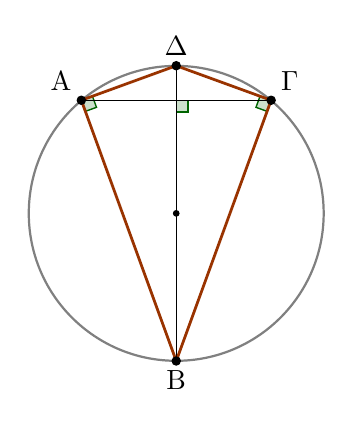
\begin{tikzpicture}[scale=.75]
\tkzSetUpLine[line width=1pt,color=black]
\tkzSetUpPoint[fill=black]

\tkzDefPoint(90:2.5){D}
\tkzDefPoint(50:2.5){C}
\tkzDefPoint(130:2.5){A}
\tkzDefPoint(270:2.5){B}

\tkzFillPolygon[fill=white](A,B,C,D)

% Find the intersection of the diagonals.
\tkzInterLL(B,D)(A,C) \tkzGetPoint{I}

\tkzMarkRightAngles[line width=0.5pt, size=.2,color=AngleClr,fill=AngleClr,fill opacity=0.2](B,I,C D,A,B D,C,B)

\tkzDefCircle[circum](A,B,C) \tkzGetPoint{O}

\tkzDrawSegments[line width=0.5pt,color=black](A,C B,D)
\tkzDrawCircle[line width=0.8pt](O,A)

\tkzDrawPolygon[color=ShapeClr](A,B,C,D)
\tkzDrawPoints[size=3](A,B,C,D)
\tkzDrawPoints[size=2](O)
\tkzLabelPoint[above left](A){$\rm A$}
\tkzLabelPoint[below](B){$\rm B$}
\tkzLabelPoint[above right](C){$\rm \Gamma$}
\tkzLabelPoint[above](D){$\rm \Delta$}

\end{tikzpicture}

\end{document}
